\documentclass[12pt,openany]{book}
\usepackage{geometry,graphicx,color}
\usepackage[dvipsnames]{xcolor}
\usepackage{mathrsfs}
\usepackage{fontspec}
\usepackage{fancyhdr}
\usepackage{mathrsfs}
\usepackage{amssymb,amsmath,mathrsfs}    
\geometry{
  a4paper,
  top=25.4mm, bottom=25.4mm,
  left=20mm, right=20mm,
  headheight=2.17cm,
  headsep=4mm,
  footskip=12mm
}
\usepackage[strict]{changepage} % 提供一个 adjustwidth 环境
\usepackage{framed} % 实现方框效果
\usepackage{tcolorbox}
\usepackage{mathpazo}% 采用 Palatino 风格字体
\usepackage[nofontspec]{newpxtext}
\tcbuselibrary{breakable,theorems}

\definecolor{winered}{rgb}{0.5,0,0}
\definecolor{structurecolor}{RGB}{122,122,142}
\definecolor{main}{HTML}{3D445F}
\definecolor{second}{HTML}{627581}
\definecolor{third}{HTML}{9D8798}

% 定义引用的颜色
\usepackage{hyperref}
\hypersetup{colorlinks = true, linktoc=all, linkcolor=black, urlcolor=winered}

% ------------------------------------------------------------%
%%%%%%%%%%颜色设置
\definecolor{formalshade}{rgb}{0.95,0.95,1} % 文本框颜色
\definecolor{Blue}{rgb}{0,0,0.5}

%%%%%%%文本框设置
\newenvironment{formal}{%
\def\FrameCommand{%
\hspace{1pt}%
{\color{Blue}\vrule width 2pt}%
{\color{formalshade}\vrule width 4pt}%
\colorbox{formalshade}%
}%
\MakeFramed{\advance\hsize-\width\FrameRestore}%
\noindent\hspace{-4.55pt}% disable indenting first paragraph
\begin{adjustwidth}{}{7pt}%
\vspace{2pt}\vspace{2pt}%
}
{%
\vspace{2pt}\end{adjustwidth}\endMakeFramed%
}


% ---------------------------------------------------------%
% 设置章形式
\usepackage{titlesec, titletoc}
\linespread{1.2} 				
\usepackage{fancyhdr}
\fancyhf{}
\renewcommand{\headrule}{\color{structurecolor}\hrule width\textwidth}
\pagestyle{fancy}
\renewcommand{\headrulewidth}{1pt}
\fancypagestyle{plain}{\renewcommand{\headrulewidth}{0pt}\fancyhf{}\renewcommand{\headrule}{}}

\fancyhead[c]{\color{structurecolor}\rightmark}
\fancyfoot[c]{\color{structurecolor}\small\thepage}

\titleformat{\chapter}[display]{\Large}
{\color{structurecolor}\filleft
\parbox{1cm}{\vbox to 1.5cm{\vfill\hbox to 4cm{\hfill\Huge \bfseries \color{structurecolor}{Chapter} \thechapter \hfill}}}}
{1ex}
{\color{structurecolor} \titlerule[2pt]\large\bfseries \filright \vspace*{1em}}
[\vspace*{1em} {\titlerule[2pt]}]

\titleformat{\section}[frame]{\normalfont\color{structurecolor}}{\footnotesize \enspace \large \textcolor{structurecolor}{\S \,\thesection}\enspace}{6pt}{\Large\filcenter \bf }


\titleformat{\subsection}[hang]{\bfseries}{\large\bfseries\color{structurecolor}\thesubsection\enspace}{1pt}{\color{structurecolor}\large\bfseries\filright}

\titleformat{\subsubsection}[hang]{\bfseries}{\large\bfseries\color{structurecolor}\thesubsubsection\enspace}{1pt}{\color{structurecolor}\large\bfseries\filright}
% ------------------------------------------------------------%
% 设置封面
\usepackage{titling}
\renewcommand*{\maketitle}{
    \begin{titlepage}
    \newgeometry{margin = 0in}
    \parindent=0pt
    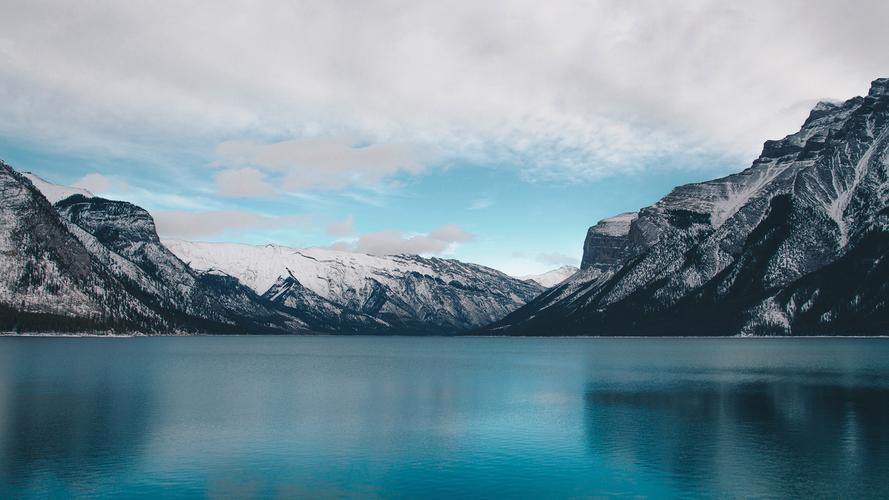
\includegraphics[width=\linewidth]{cover}
    \vfill
    \begin{center}
        \parbox{0.618\textwidth}{
        \hfill {\bfseries \Huge \thetitle} \\[0.6pt]  
        \rule{0.618\textwidth}{4pt} \\ 
    }
    \end{center}
    \vfill
    \begin{center}
        \parbox{0.618\textwidth}{
        \hfill\Large
          \begin{tabular}{r|}
          Author: \theauthor \\ 
          Date: \thedate \\
        \end{tabular}
        }
    \end{center}
    \vfill
    \begin{center}
        \parbox[t]{0.7\textwidth}{\centering }
    \end{center}
    \vfill
\end{titlepage}
\restoregeometry
\thispagestyle{empty}
}
% ------------------------------------------------------------%


\title{GW Scattering Notes}
\author{Lingyu Xia}
\date{\today}

\begin{document}
\frontmatter

\maketitle
\setcounter{page}{0}
\tableofcontents

\newpage

\mainmatter
\pagenumbering{arabic}
%%%%%%%%%%%%%%%%%%%%%%%%
\chapter{Scattering}

\par We would like to talk about the quantum scattering theory at this chapter. Different from the classical scattering theorem, we need to consider the quantum property of scattered particles, and obtain the scattering potential distribution by Schrödinger equation.

\section{The introduction of scattering}


\par As for the quantum scattering, we list fundamental assumptions:
\begin{itemize}
    \item Since the scattering phenomenon is observed away from the scattering center, we give the $r\rightarrow \infty$condition
    \item We assume that the scattering  is elastic so that the energy and wave vector won't change 
\end{itemize}

So we give the formula for the differential cross-section of scattering from Schrödinger equation below. Let us start from Schrödinger equation
\begin{align}
    \frac{\hbar^{2}}{2m}\nabla ^{2}\psi+U(\mathbf{r})\psi=E \psi
\end{align}

We write it as a wave equation, and then using our assumptions, so we get

\begin{align}
    \nabla^{2}\psi+k^{2}\psi=0
\end{align}
where $k^{2}=\frac{2mE}{\hbar^{2}}$, its solution is $e^{i{\mathbf{k}}\cdot {\mathbf{r}}}$. As for the scattering system, we separate the wave into two parts, one is a plane wave coming from a distance, and the other is a scattered wave. The solution should be a superposition of the two kinds of wave

\begin{align}
    \psi \overset{r\rightarrow \infty}{\rightarrow}A\left[e^{ikz}+f(\theta)\frac{e^{ikr}}{r}\right]
\end{align}


Then the probability of an incident particle in a direction is 

\begin{align}
    |\psi|dV=|Ae^{ikz}|^{2}(vdt)d\sigma=|A|^{2}(vdt)d\sigma
\end{align}
The probability of an outgoing particle appearing in an azimuth is

\begin{align}
        |\psi|dV=\left|Af(\theta)\frac{e^{ikr}}{r}\right|(vdt)r^{2}d\Omega=|A^{2}|f|^{2}(vdt)d\Omega
    \end{align}
The equation of differential scattering cross section can be obtained because the continuity conditional probability is
\begin{formal}
    \begin{align}
        D(\theta)\equiv\frac{d\sigma}{d\Omega}=|f(\theta)|^{2}
    \end{align}
\end{formal}

\section{The partial wave expansion}

Because of the spherical symmetry, we consider the separation of variables method

\begin{align}
    \psi(e,\theta,\varphi)=R(r)Y_{lm}(\theta,\varphi)
\end{align}
where $Y_{lm}(\theta,\varphi)$ is harmonic spherical function.

As for the function $u(r)=rR(r)$, it satisfies following equation

\begin{formal}
    \begin{align}
        \frac{d^{2}u}{de^{2}}+\left\{\frac{2m}{\hbar^{2}}[E-V(r)]-\frac{l(l+1)}{r^{2}}\right\}u=0\quad (l=0,1,2,...)
    \end{align}
\end{formal}

Then on the basis of our assumptions, we keep simplifying this equation. When $r\rightarrow \infty$, $V(r)\rightarrow 0$, and $\frac{l(l+1)}{r^2}u$ can also be neglected, then we have

\begin{align}
    \frac{d^{2}u}{dr^{2}}+k^{2}u=0
\end{align}

Its general solution is $u=Ae^{ikr}+Be^{-ikr}$, so the original function is 

\section{Born approximation}



\end{document}